\chapter{Simulation results}


\section{Case tests presentation}

In this section we dedicate some words to give informations about what kind of input file FEMOS get in input and what files it produces.
Basically all .tdr format are accepted by FEMOS code. For our simulation it was possible used synopsis tools. More precisely the device design was performed with SDE and the mesh generator used 
was SNMESH. About output we produce .xmf files easly visible with paraview.

 We focus our tests over three main structures: diode, diode inside an oxide box and a transistor mos.  
Here we presents the geometry tested and some mesh pattern used.

\begin{figure}[!h]
\subfloat[]
{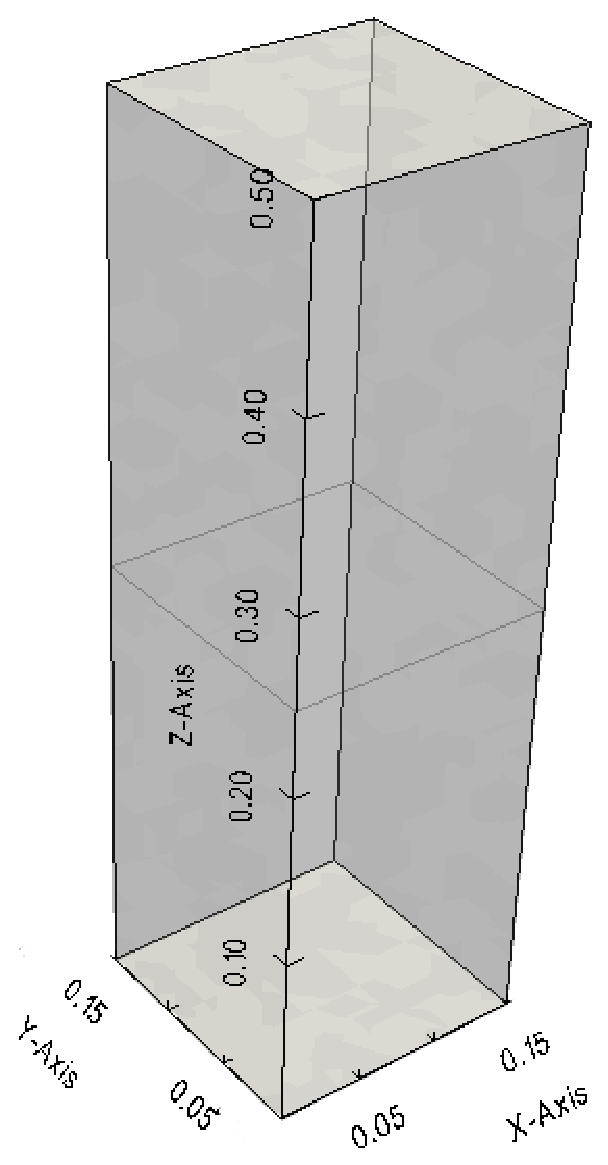
\includegraphics[height = 5.5cm,width = 3cm]{Casitest/DominioNP}}
\psp{10}
\subfloat[]
{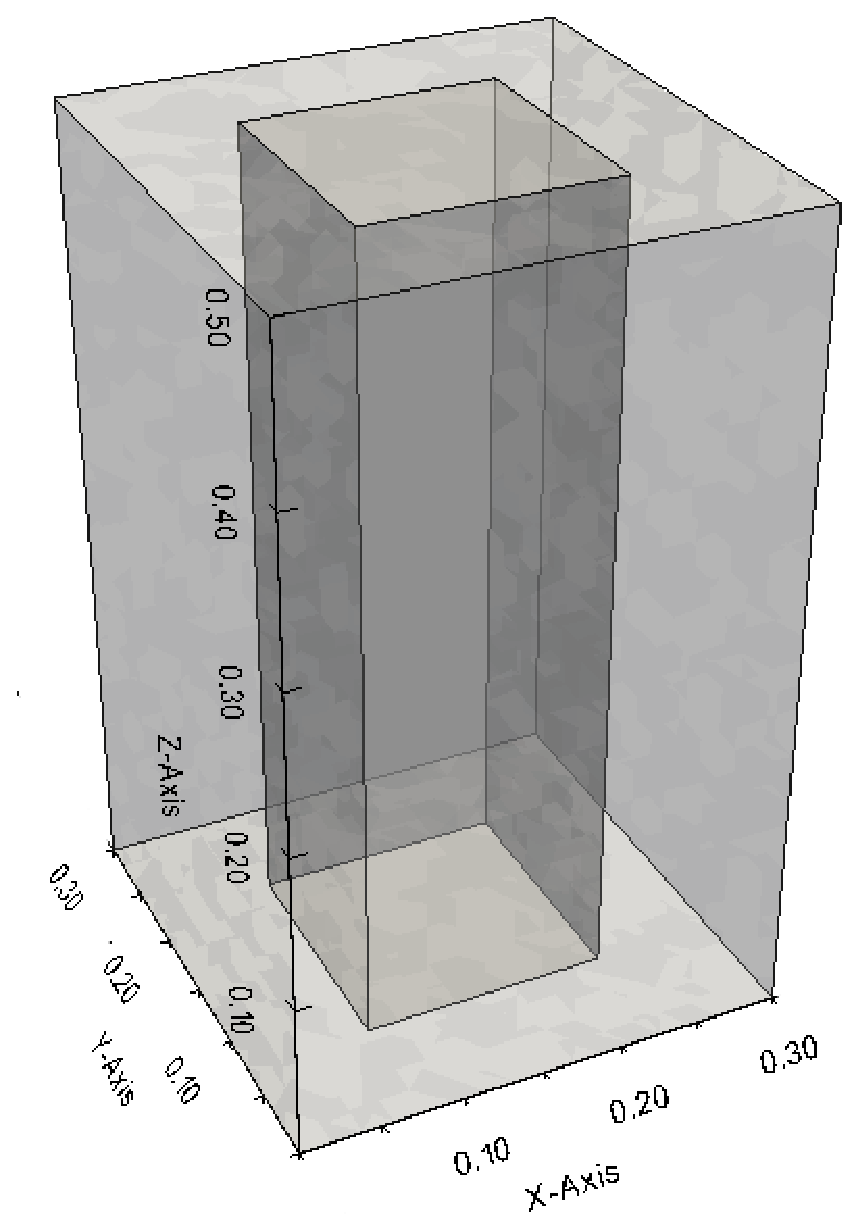
\includegraphics[height = 5.5cm,width = 3cm]{Casitest/DominioNPOX}}
\psp{10}
\subfloat[]
{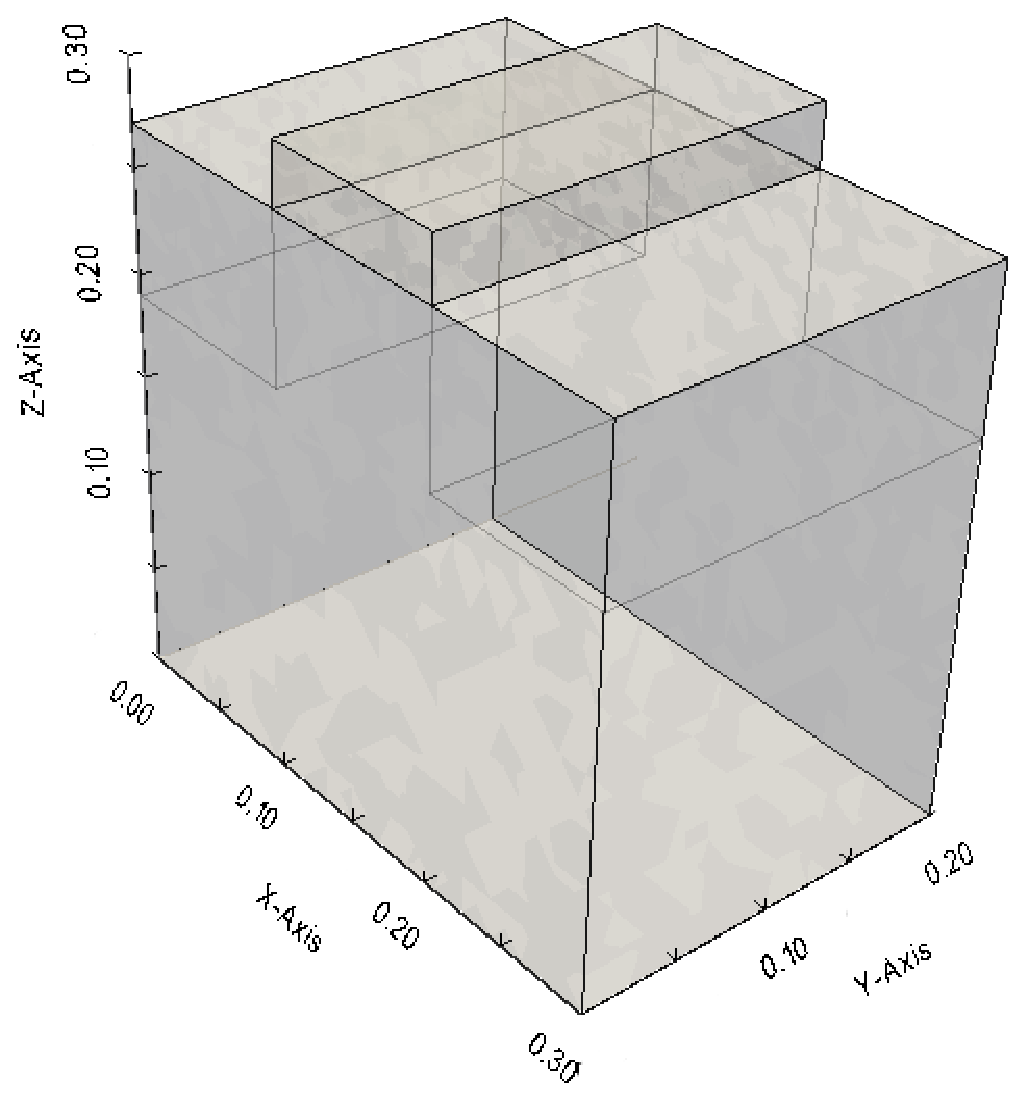
\includegraphics[height = 5.5cm,width = 4cm]{Casitest/DominioMOS}}
\end{figure}

 For everyone of these case test we investigated different doping concentration and distribution (like abrupt or gauss profile), multiple generation/recombination and mobility models applyed, ....
Results are always checked with the SDEVICE simulation ...

\clearpage


\begin{figure}[!h]
\centering
\subfloat[][\emph{Mesh}]
{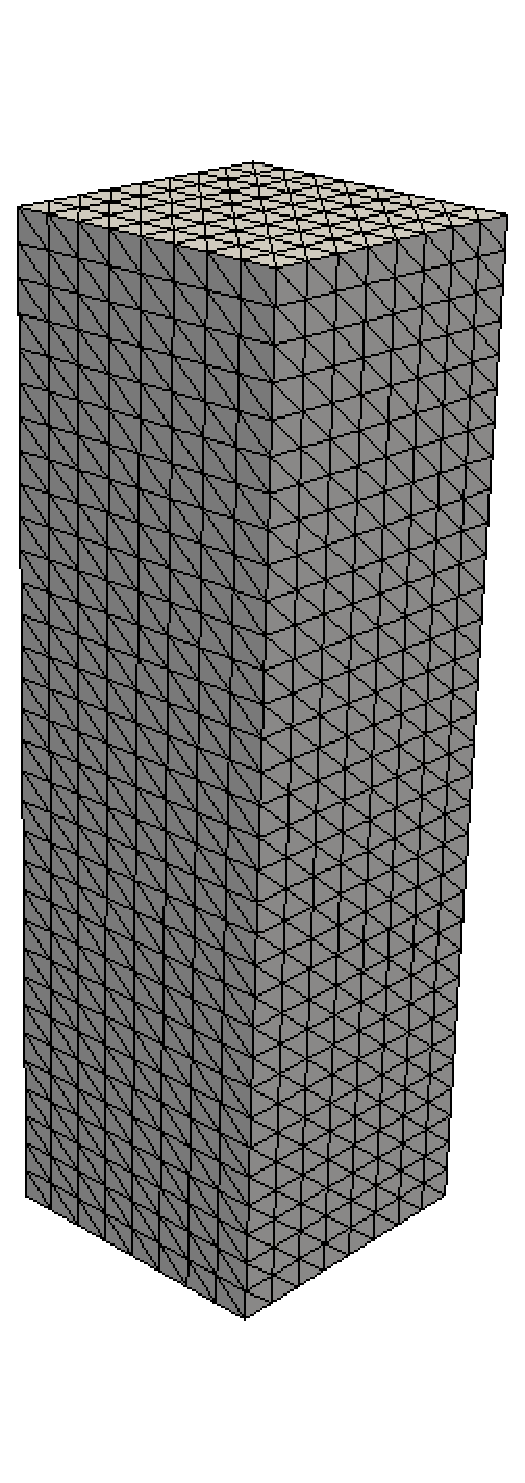
\includegraphics[scale=0.36]{Strutture/DiodeMesh}}
\hspace{2.5cm}
\subfloat[][\emph{Doping concentration}]
{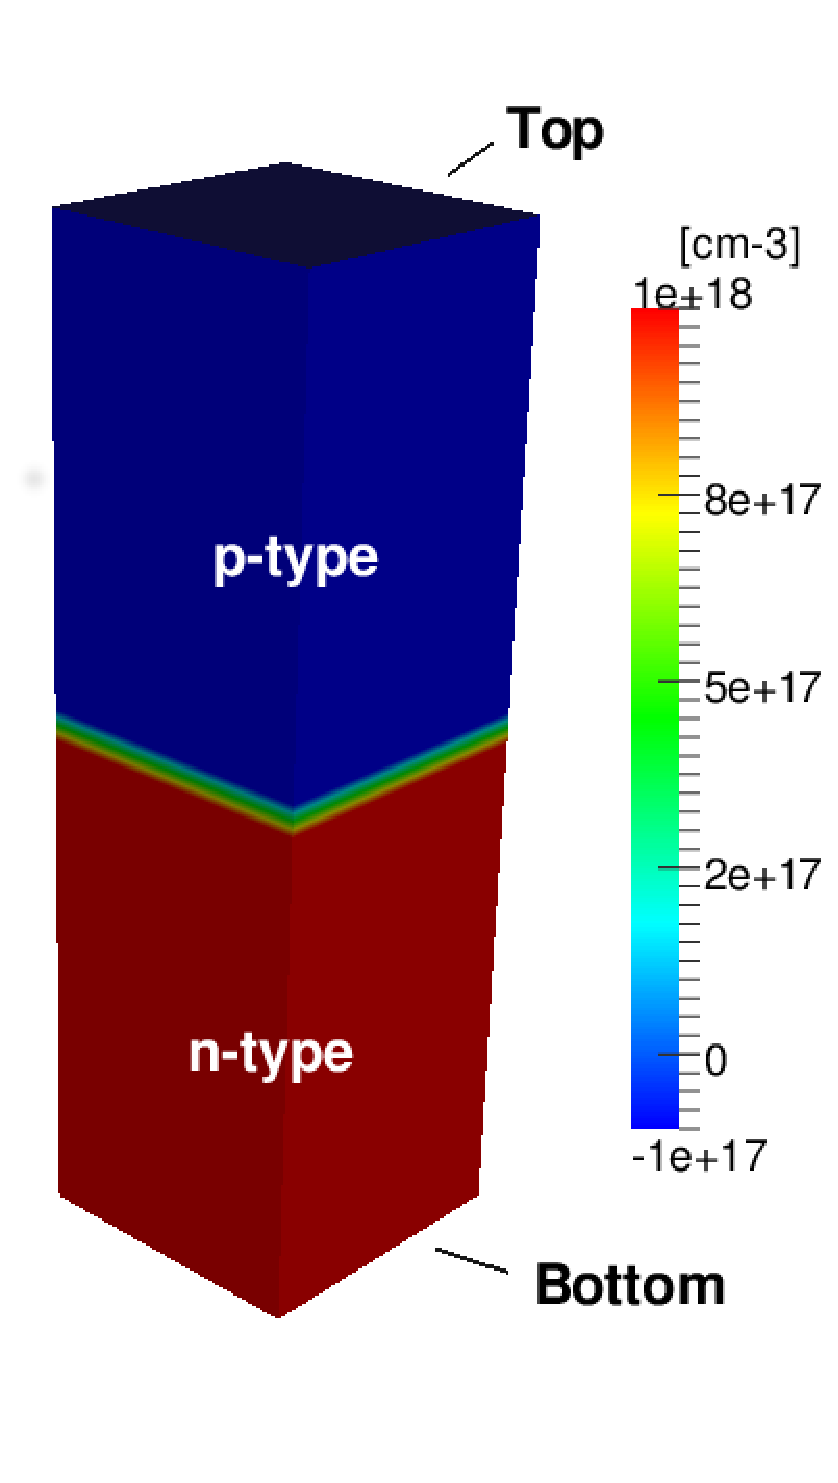
\includegraphics[scale=0.35]{Strutture/Diode1817}}
\caption{Geometry of case test Diode.}
\end{figure}

\begin{figure}[!h]
\centering
\subfloat[][\emph{Mesh}]
{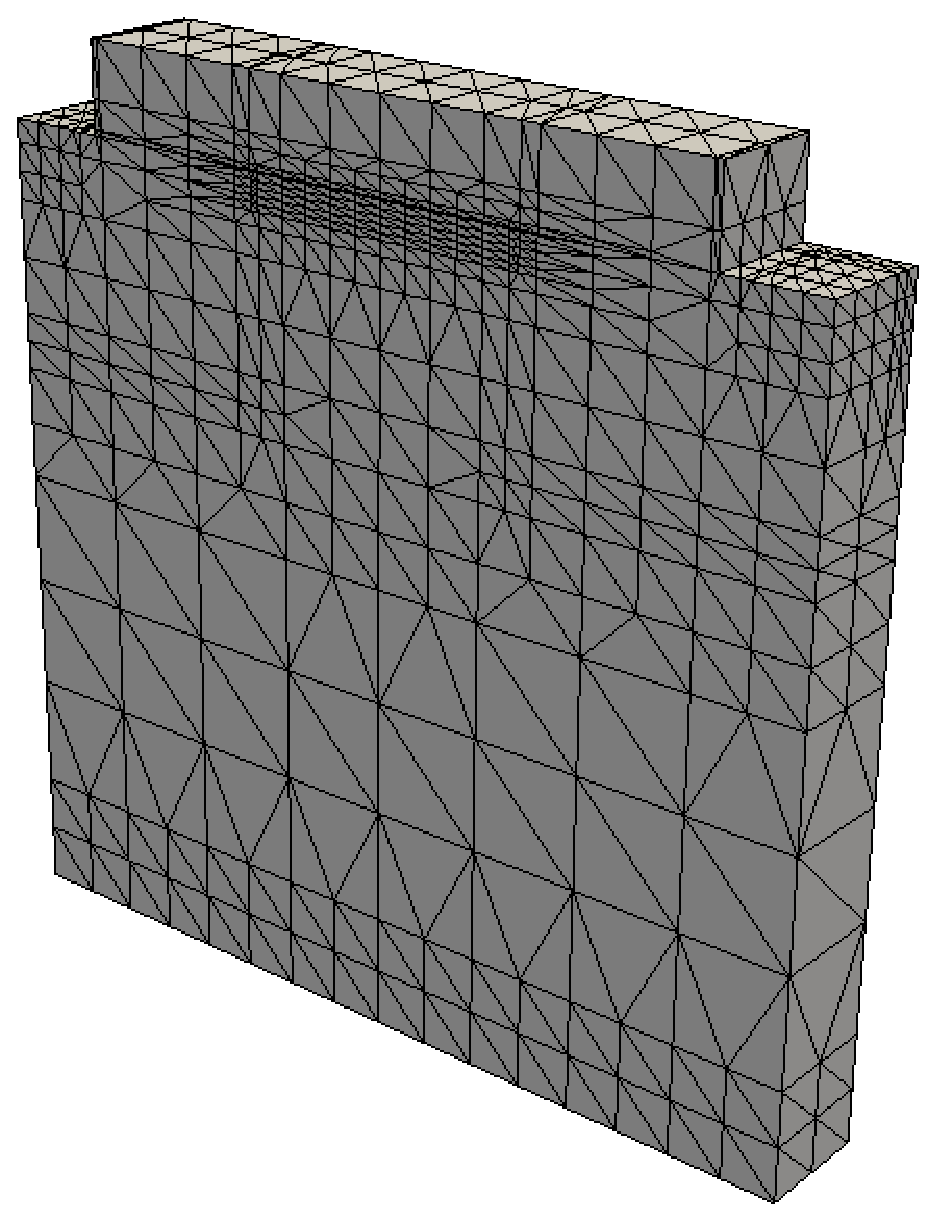
\includegraphics[scale=0.32]{Strutture/MosMesh}}
\hspace{1.5cm}
\subfloat[][\emph{Doping concentration}]
{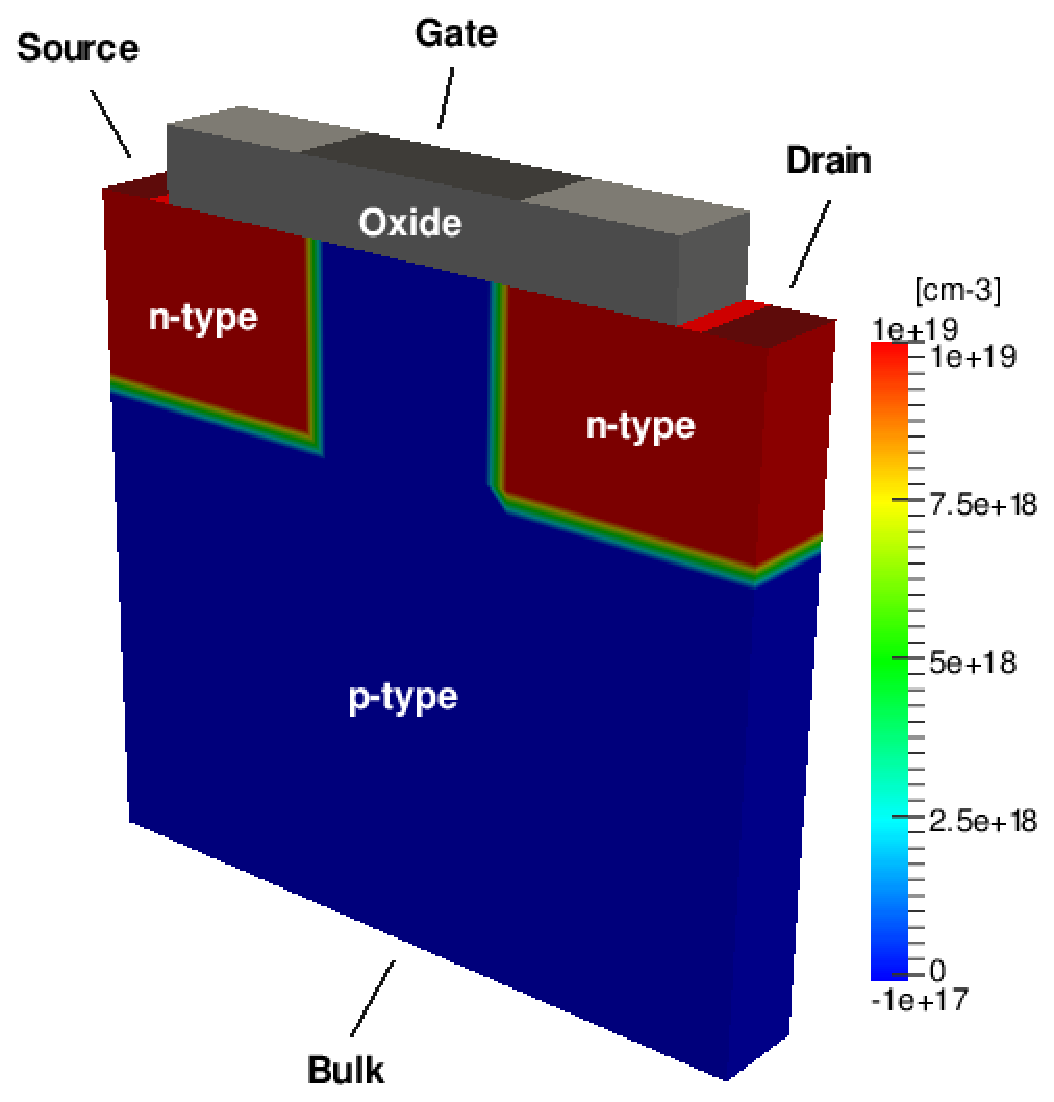
\includegraphics[scale=0.38]{Strutture/MosDoping191719}}
\caption{Geometry of case test MOS n-channel.}
\end{figure}
